\chapter{Estado del arte}
\label{ch:estado}

\section{Realidad aumentada}
La realidad aumentada es una tecnología que permite añadir información virtual al mundo real a través de un dispositivo, es decir, permite mostrar en conjunto el mundo real con objetos virtuales en éste, por lo que no pretende crear un mundo virtual, sino complementar al mundo real con más información. Una de las primeras definiciones de realidad aumentada fue dada por Ronald Azuma en 1997, que dice que la Realidad Aumentada es cualquier sistema que combine elementos reales y virtuales, que sea interactivo en tiempo real y que sea registrado en tres dimensiones. \cite{azuma}

\section{DIFERENCIAS ENTRE REALIDAD AUMENTADA, REALIDAD VIRTUAL Y REALIDAD MIXTA}
Realidad virtual: Es una tecnología completamente inmersiva que consiste en convencer a tus sentidos de que estas en otro mundo que no es el real, es un mundo virtual. Usando un dispositivo que se coloca en la cabeza, la realidad virtual permite disfrutar de un mundo de imágenes y sonidos generado por ordenador en el que puedes manipular objetos, y moverte por dicho mundo usando controladores hápticos conectados a un ordenador o a una consola. [2]

Realidad aumentada: Es una tecnología que superpone información digital sobre elementos del mundo real. El elemento central es el mundo real, pero lo mejora con otros detalles digitales, complementando así la realidad. [2]

Realidad mixta: Es una tecnología que hace converger el mundo real y elementos digitales. En esta puedes interactuar y manipular tanto elementos físicos como virtuales. La realidad mixta te permite sumergirte en el mundo que te rodea incluso cuando tú interactúas con el entorno virtual usando tus propias manos. Esta tecnología te permite tener un pie en el mundo real y el otro en un lugar imaginario. [2]

\section{APLICACIONES DE LA REALIDAD AUMENTADA}
Medicina: La realidad aumentada puede aportar grandes avances a la medicina, ya que permite la visualización en 3D de objetos que bien pueden ser órganos o partes del cuerpo en el mundo real, por lo que puede facilitar a los doctores muchas tareas que requieran el estudio de modelos 3D. Por ejemplo, los doctores pueden utilizar la realidad aumentada con el objetivo de prepararse para una operación, o simplemente para tareas de visualización médica, de igual manera que actualmente se utilizan los TAC o las resonancias magnéticas, pero los datos obtenidos con dichos escáneres se convertirían en modelos 3D que son mucho más sencillos de explorar que un conjunto de imágenes 2D. También se podría utilizar la realidad aumentada con el objetivo de entrenamiento para cirujanos que se están

\newpage
Como podemos ver en la imagen \ref{mireferencia}

\begin{figure}
  \centering
  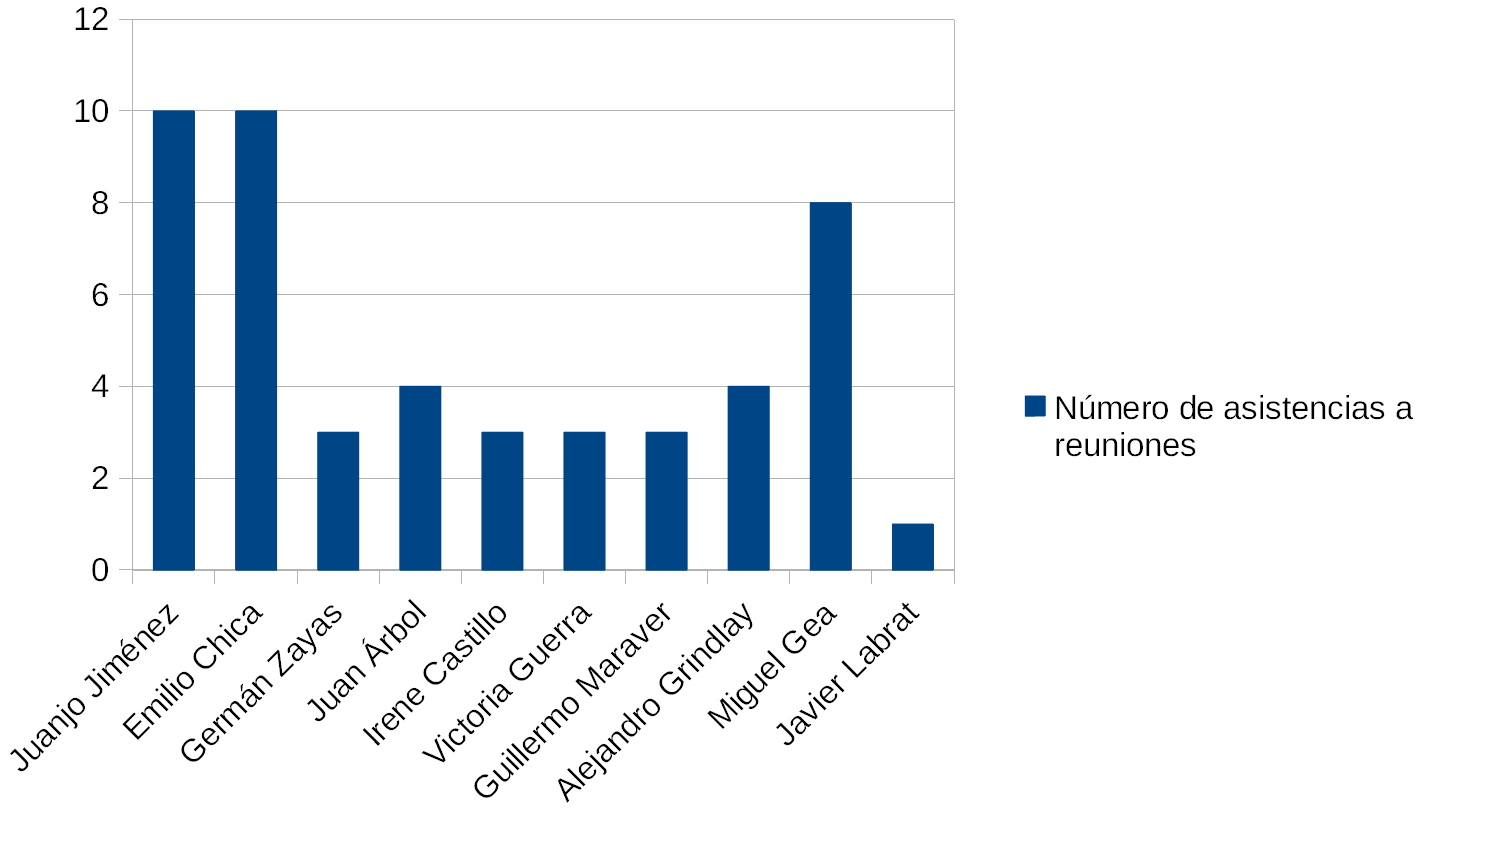
\includegraphics{asistencias}
  \caption{ejemplo de caption}
  \label{mireferencia}
\end{figure}

\begin{figure}
    \centering
    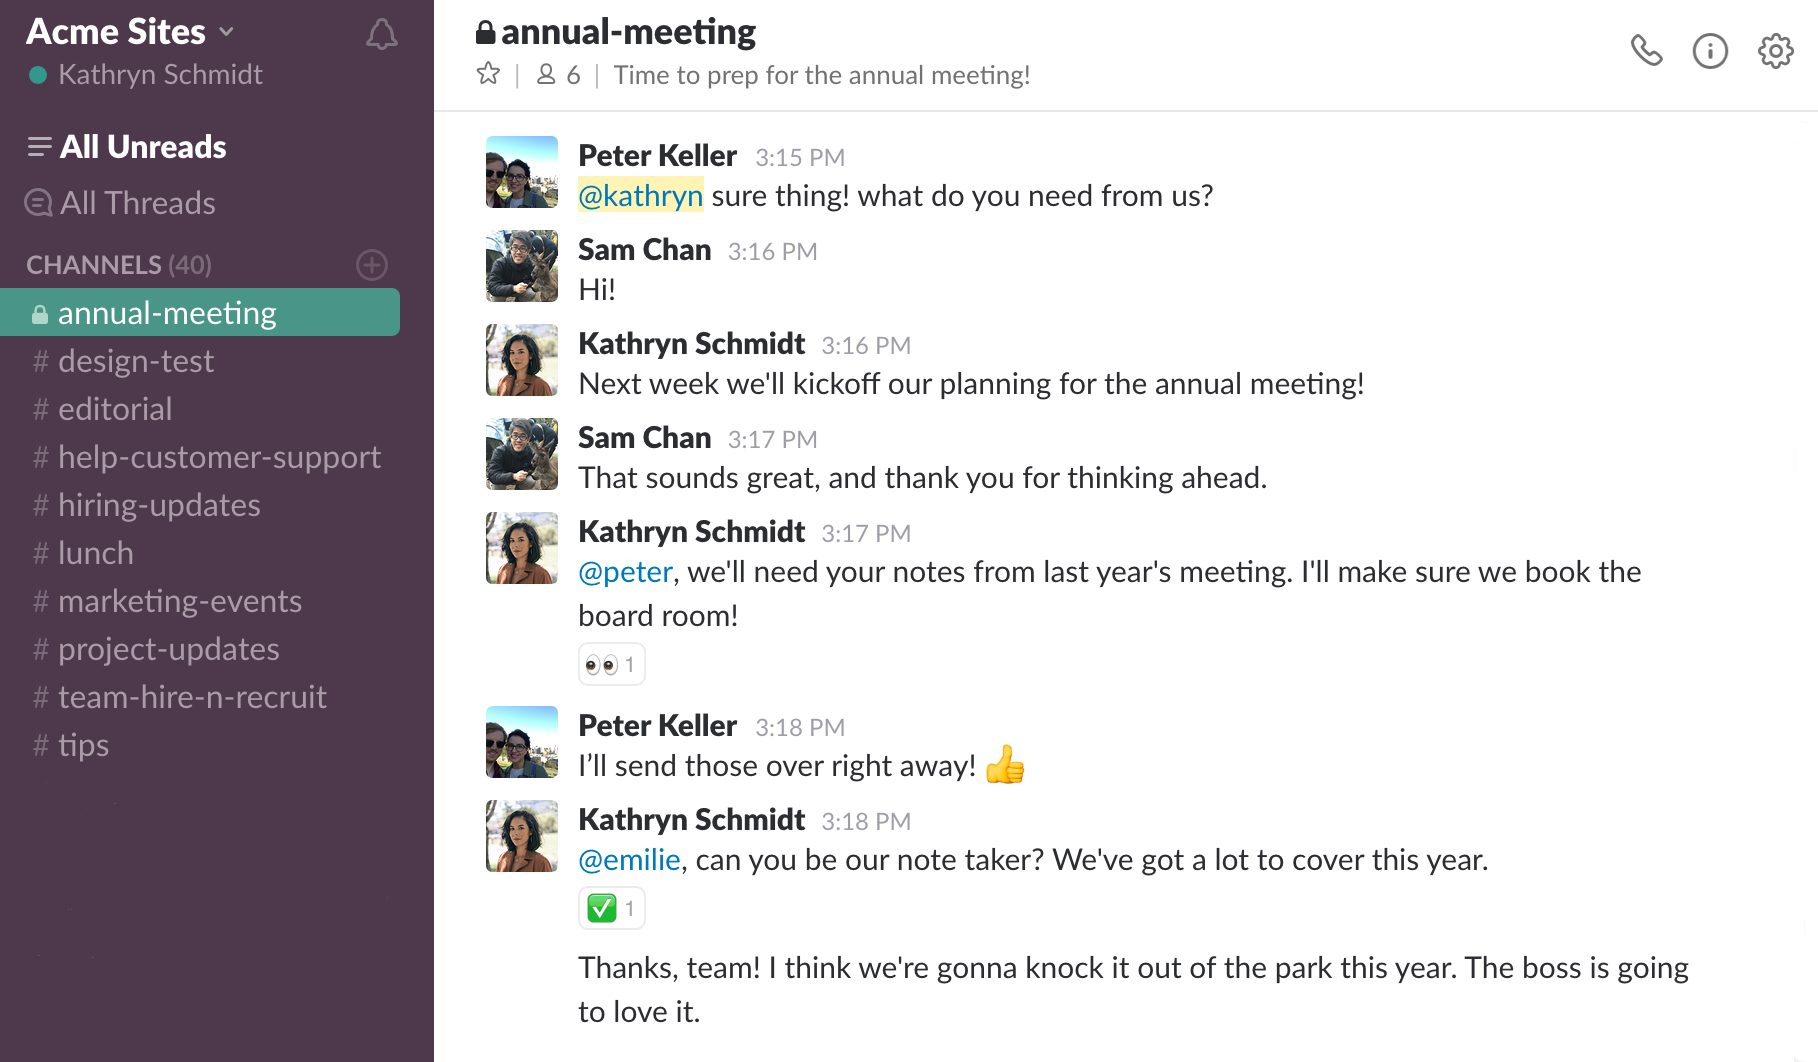
\includegraphics[scale=0.2]{slack}
    \caption{Pantalla principal de Slack - \textcopyright\ Slack}
    \label{slackimage}
\end{figure}

\begin{table}
    \begin{center}
        \begin{tabular}{|p{4.5cm}|p{6.5cm}|}
            \hline
                \rowcolor{Gray}\multicolumn{1}{|c|}{\textbf{Integrante}}
                & \multicolumn{1}{|c|}{\textbf{Ocupación}} \\
            \hline
                Juan Árbol Gutiérrez & Estudiante de CC.EE. y Empresariales \\
            \hline
                Irene Castillo Pardo & Estudiante de Comunicación y Audiovisuales \\
            \hline
                Emilio Chica Jiménez & Estudiante de Ingeniería Informática \\
            \hline
                Victoria Guerra Molina & Estudiante de Comunicación y Audiovisuales \\
            \hline
                Juan José Jiménez García & Estudiante de Ingeniería Informática \\
            \hline
                Javier Labrat Rodríguez & Estudiante de Ingeniería Informática \\
            \hline
                Germán Zayas Cabrera & Estudiante de Bellas Artes \\
            \hline
                Miguel Gea Megías & Profesor de Ingeniería Informática \\
            \hline
                Guillermo Maraver Tarifa & Profesor de CC.EE. y Empresariales \\
            \hline
                Alejandro Grindlay Moreno & Profesor de Ingeniería Civil \\
            \hline
        \end{tabular}
        \caption{Integrantes del proyecto multidisciplinar SmartU}
        \label{miembrossmartu}
    \end{center}
\end{table}
